\RequirePackage{luatex85}
\documentclass[tikz, border=10pt]{standalone}

\usepackage[compat=1.1.0]{tikz-feynman}

\begin{document}

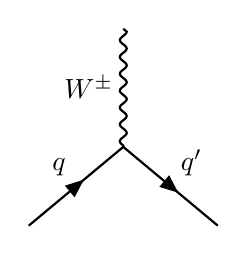
\begin{tikzpicture}[thick]
 \begin{feynman}
  \vertex (origin);
  \vertex [above=1.5cm of origin] (W);
  \vertex [below left=1cm and 1.2cm of origin] (q1);
  \vertex [below right=1cm and 1.2cm of origin] (q2);
  \diagram* {
  (origin) -- [boson, edge label={\(W^{\pm}\)}] (W),
  (q1) -- [fermion, edge label={\(q\)}] (origin),
  (origin) -- [fermion, edge label={\(q'\)}] (q2),
  };
 \end{feynman}
\end{tikzpicture}
\end{document}
